\chapter{Scientific Background}
This chapter provides a theoretical background for the topics addressed in this thesis.
It introduces the fundamental physical processes and structures of Active Galactic Nuclei (AGN), with a particular focus on the properties of the Broad-Line Region (BLR), which plays a central role in this work. The concept of AGN unification, the different observational classifications, and the variability of AGN are outlined.Furthermore, reverberation mapping is discussed in detail, as it serves as the main analysis method in this thesis. It is a powerful tool to probe the geometry and kinematics of the BLR and to estimate the mass of the central supermassive black hole.In the final section of this chapter, an overview of Bowen fluorescence is provided, as this process may account for some spectral features that will be discussed in the following analysis.

\section{Active Galactic Nuclei}

What are Active Galactic Nuclei (AGN)? They represent a class of galaxies that are among the brightest and most energetic objects in the known universe, with bolometric luminosities ranging from $10^{41}$ to $10^{48} \ \mathrm{erg \ s^{-1}}$, surpassing typical galaxies by many orders of magnitude \parencite{peterson1997introduction}.\
This enormous emission originates from the central region of the AGN, which outshines the stars of its so-called host galaxy. It is powered by matter accreting onto the central supermassive black hole (SMBH) in the form of an accretion disk \parencite{shakura1973black}.\\
To better understand the physical nature of AGN, it is important to examine their observational characteristics and internal structure. AGN emit radiation across the entire electromagnetic spectrum, and their spectral features provide crucial information about the physical conditions and kinematics in the central regions.\\
The following sections present the main components of AGN, introduce the unification model that links different AGN types, and describe commonly used classification schemes. Particular attention is given to the variability of AGN, which plays a central role in the reverberation mapping analysis carried out in this thesis.

\subsection{Spectral Features}

AGNs emit radiation across the entire electromagnetic spectrum. A typical AGN exhibits strong X-ray and radio emission, as well as non-stellar ultraviolet and optical continua, along with both broad and narrow emission lines. However, not every AGN displays all of these features, as will be discussed in more detail later \parencite{peterson1997introduction}.

\subsection{Structur of an AGN}

\begin{figure}[!ht]
	\centering
	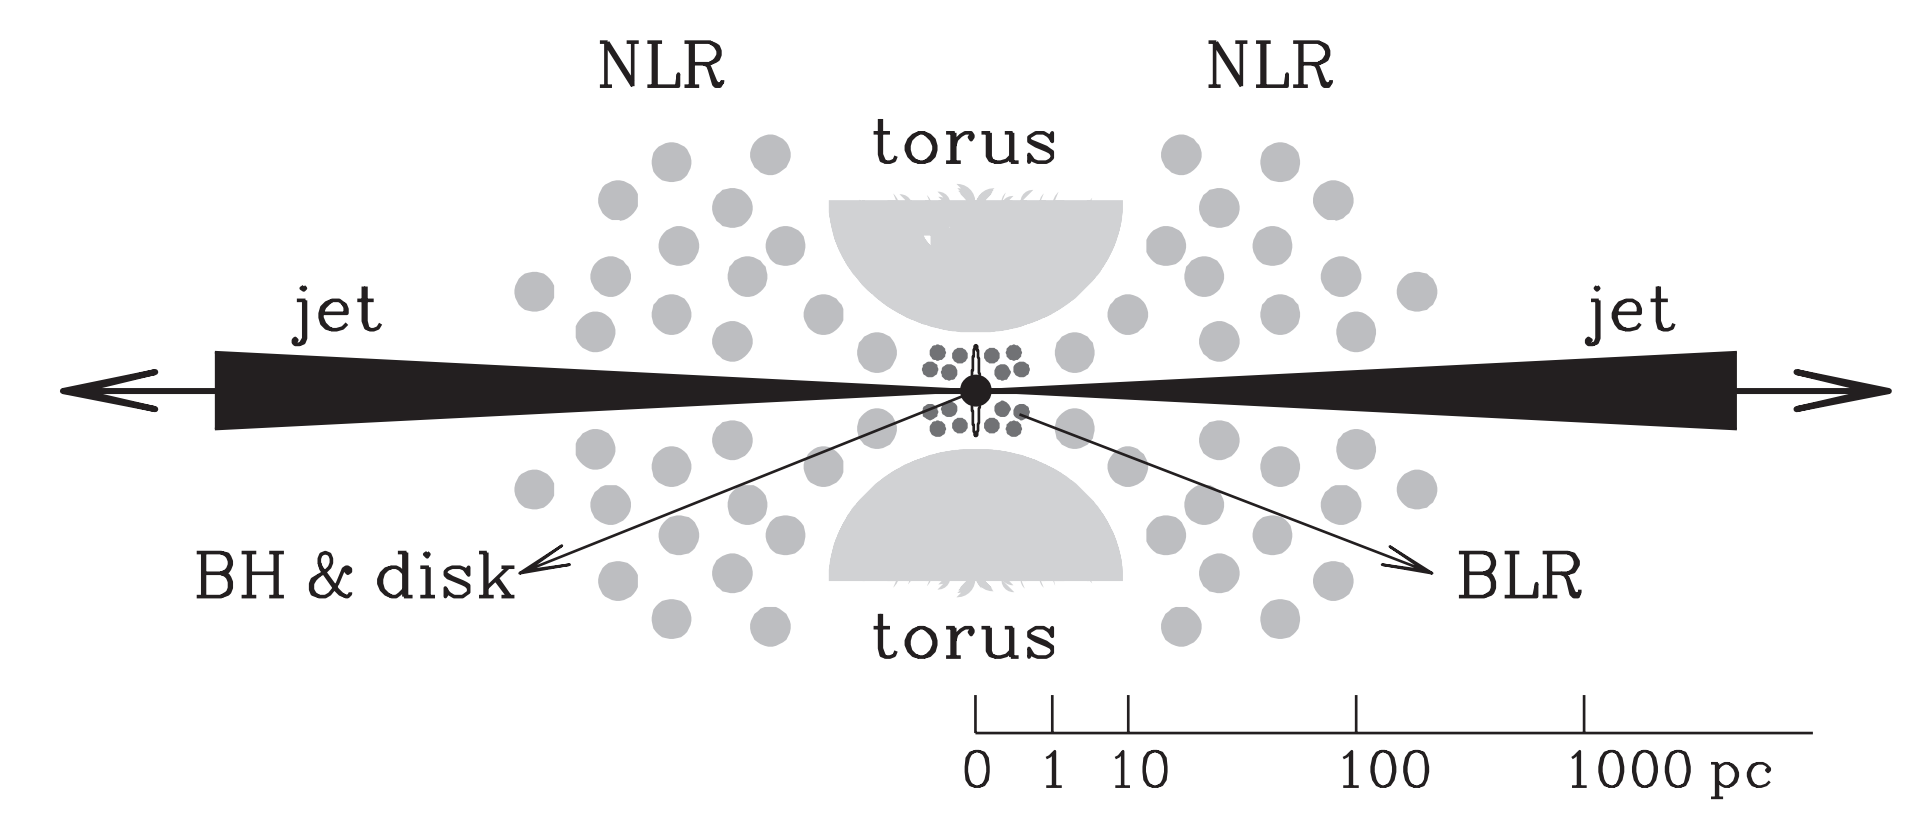
\includegraphics[width=0.8\textwidth]{pictures/Chapter2/AGN_standard_paradigm.png}
	\caption{Different components of an AGN. Adapted from \textcite{mo2010galaxy}.}
	\label{fig:agn_structure_mo}
\end{figure}


\subsection{Unification Model}
Figure \ref{fig:agn_sed} shows the unification model of an AGN. 
As illustrated an AGN is powered by a supermassive black hole surrounded by several distinct regions. Closest to the black hole is the accretion disc, whose hot, optically thick gas emits the thermal “Big Blue Bump” in the optical/UV bands \parencite{peterson1997introduction}. Encircling the disc is the Broad-Line Region (BLR), a compact area of dense clouds orbiting at thousands of kilometers per second, which produces the broad emission lines. Outside the BLR lies the dusty torus, a toroidal structure of cooler gas and dust that can obscure the inner regions when viewed edge-on \parencite{antonucci1993unified}. Beyond the torus, the more extended Narrow-Line Region (NLR) emits narrower lines from slower gas at distances of hundreds of parsecs. In radio-loud AGN, powerful relativistic jets emerge perpendicular to the disc plane, accelerating particles to near-light speeds and generating strong radio emission \parencite{urry1995unified}.


\begin{figure}[!ht]
	\centering
	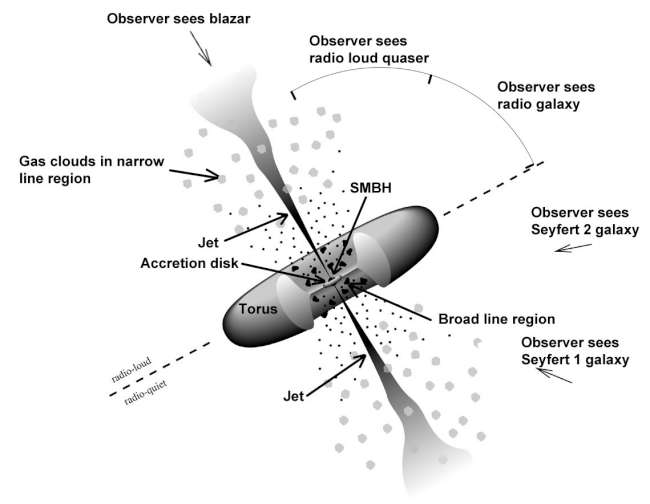
\includegraphics[width=\textwidth]{pictures/Chapter2/AGN_unified_model.jpg}
	\caption{Unification model of an AGN \parencite{fermi2025figure1}.}
	\label{fig:agn_sed}
\end{figure}

\subsection{Classification}

AGNs can be broadly grouped into so called Seyfert galaxies, quasars and radio galaxies. Seyfert galaxies are further subdivided, based on the width of their optical emission lines and radio properties. Seyfert 1 Galaxies show broad emission lines, while Seyfert 2 Galaxies show only narrow emission lines, narrow-line Seyfert 1 galaxies (NLS1), low-ionization nuclear emission-line regions (LINERs), and BL Lac objects or blazars \parencite{antonucci1993unified,urry1995unified}.\\\\

\subsection{Variability}

\section{Reverberation Mapping}


\subsection{Principle}


The main focus of this work was to perform a classic reverberation analysis of NGC 4593, with a focus on the broad line region (BLR) and its geometry around the central supermassive black hole (SMBH).\\\\
This type of analysis aims to measure the time lag $\tau$ between the variable continuum and the emission line response, in order to determine the spatial scale and structure of the BLR. By observing these variations over time and analyzing the delayed response of the broad lines, it is possible to learn more about the geometry and dynamics of the BLR and to estimate the mass of the SMBH.\\\\
Reverberation mapping (RM) is based on the strong correlation between a variable continuum emission $C(t)$ and the emission line flux $L(\nu, t)$ \parencite{horne2021space}. This correlation originates from the photoionization of gas clouds in the BLR by the central continuum source. As the continuum changes, the emission lines react in a similar way, but with a time delay $\tau$, because of the distance between the central source and the BLR. This delay corresponds to the time it takes for light to travel from the central source to the BLR.\\\\

\subsection{Transferfunction}

\subsection{Cross-Correlation Function}

\subsection{Black-Hole Mass}

\section{Bowen Fluorescence}